\documentclass[10pt]{article}

\usepackage{times}
\usepackage{mathptmx}
\usepackage{amsmath}
\usepackage{mathtools}
\usepackage{graphicx}
\usepackage{epstopdf}

\setlength\parindent{0pt}


\raggedbottom
\sloppy

\title{Time-discrete Stochastic Signals\\
\emph{TSDT14}}

\author{David Habrman \\ davha227, 920908-2412\\
Jens Edhammer \\ jened502, 920128-5112 }

\date{\today}

\begin{document}

\maketitle

\section{Introduction}
This is a laboration report in signal theory (TSDT14). It consists of three studies.

\subsection{Study 1 – Modelling Signals}
Study 1 involves analyzing the power spectral density (PSD) and auto correlation function (ACF)
of noise filtered through two diffrent filters. One close to ideal and one simple low pass filter.
The ACF and PSD were first theoretically calculated and then estimated.
The ACF was estimated using Blackman-Tukey's- and Barlett's -estimate and the
PDF was estimated using periodograms, averaged periodograms and smoothed periodograms.

\subsection{Study 2 – Non-LTI-systems}
In study 2 we use noise filtered through an ideal filter and use it as input to three different non-LTI-systems.
This gives us output signals for which the PSD is computed, both theoretically and by using the estimation methods
from study 1. The  amplitude distribution is also computed. Both the PSD and the  amplitude distribution are then used
to demonstrate that the systems are non-LTI.

\subsection{Study 3 – Special Operations}
In study 3 we use the filtered noise from study 2 as input to two different systems.
This gives us output signals for which the PSD is computed theoretically and estimated using
periodograms. The theoretical and estimated PSD is then compared.

\subsection{Notation}
The following notations will be used. \\
PSD - Power Spectral Density \\
ACF - Auto correlation function \\
$\hat{r_y}$ - Estimated ACF of signal y. \\
$\hat{R_y}$ - Estimated PSD of signal y. \\
WGN - White Gaussian Noise\\
Sq - Shorthand for squarer\\
Hw - Shorthand for half-wave rectifier\\
Am - Shorthand for AM-SC modulator\\
$\Omega_0$ - Carrier frequency\\

\section{Study 1 – Modelling Signals}
\subsection{Method}

White Gaussian noise is used in this study. It was filtered through the two
 filters described in equation~\ref{eq:simpleH} and equation~\ref{eq:idealH},
  to produce our signal $y$.
 The ideal filter is approximated by a highorder Butterworth lowpass filter.

\begin{equation}
  \label{eq:simpleH}
  H[\theta]_{simple} =\frac{1-a}{1-ae^{-j2\pi\theta }}
\end{equation}

\begin{equation}
  \label{eq:idealH}
  H[\theta]_{ideal} =rect(\frac{\theta}{2\theta_0} )
\end{equation}

\subsubsection{Theoretical ACF and PSD}
PSD of WGN is constant and our WGN has a variance of one. Due to this the PSD
of our noise, $R_x$, is chosen to one.
The PSD of the filtered WGN is then calculated using equation~\ref{eq:PSDformula}.

\begin{equation}
  \label{eq:PSDformula}
  R_y[\theta] = R_x|H(\theta)|^2;
\end{equation}

The ACF can be calculated using inverse fourier transform, see equation~\ref{eq:ACFformula}.

\begin{equation}
  \label{eq:ACFformula}
  r_y[n] = \mathcal{F}^{-1}\{R_y\}[n]
\end{equation}



\subsubsection{Estimation of ACF and PSD}
The ACF was estimated using Blackman-Tukey's- and Barlett's -estimate.
This was done using equation~\ref{eq:BmanT} and equation ~\ref{eq:Blett}.

\begin{equation}
\label{eq:BmanT}
\hat{r}_y[k] =
\begin{cases}
    \frac{1}{N-|k|}\sum_{n=0}^{N-|k|-1}r_x[n+|k|]r_x[n],& \text{if } |k|< N\\
    0,              & \text{elsewhere}
\end{cases}
\end{equation}


\begin{equation}
\label{eq:Blett}
\hat{r}_y[k] =
\begin{cases}
    \frac{1}{N}\sum_{n=0}^{N-|k|-1}r_x[n+|k|]r_x[n],& \text{if } |k|< N\\
    0,              & \text{elsewhere}
\end{cases}
\end{equation}

The PSD was estimated using periodograms, averaged periodograms
and smoothing. The raw periodogram was calculated by taking the fouriertransform
of the estimated ACF.
Averaged periodograms was done by calculating a mean of the periodogram inside
an interval and repeating this for all samples. The averaged periodogram was
then set to the mean inside each interval.

The smoothed periodogram was done by first multiplying the estimated ACF with a
 suitable window and then using the fourier transform to get the estimated PSD,
 see equation~\ref{eq:win}. This can be viewed as a form of moving average in the fourier-domain.

 \begin{equation}
 \label{eq:win}
 \hat{R}_{y,smoothed}[\theta] = \mathcal{F}\{\hat{r}_yw[k]\}
 \end{equation}



\subsection{Result and conclusion}

Noted in equation~\ref{eq:ACFsimple} is the theoretically calculated functions
for the ACF for the simple filter and equation~\ref{eq:ACFideal} for the close
to ideal filter.
Equation~\ref{eq:PSDsimple} does the same for the simple filter's PSD
and equation~\ref{eq:PSDideal}, the close to ideal filter's PSD.

\begin{equation}
  \label{eq:ACFsimple}
  r_{y,simple}[n] = R_x\frac{(1-a)}{(1+a)}a^{|n|};  |a| < 1
\end{equation}

\begin{equation}
  \label{eq:PSDsimple}
  R_{y,simple}[\theta] =  R_x|\frac{1-a}{1-ae^{-j2\pi\theta}}|^2;
\end{equation}

\begin{equation}
  \label{eq:ACFideal}
  r_{y,ideal}[n] = R_x2\theta_{0}sinc[n2\theta_0];
\end{equation}

\begin{equation}
  \label{eq:PSDideal}
  R_{y,ideal}[\theta] = R_xrect[\frac{\theta - k}{2\theta_0}]
\end{equation}


The theoretical functions for the ACF and PSD for $y_{simple}$ are presented
in figure~\ref{fig:TheoACFsimple} and figure~\ref{fig:TheoPSDsimple}.
The functions for $y_{ideal}$ are presented in figure~\ref{fig:TheoACFideal} and
figure~\ref{fig:TheoPSDideal}.



\begin{figure}[!hp]

    \begin{center}
      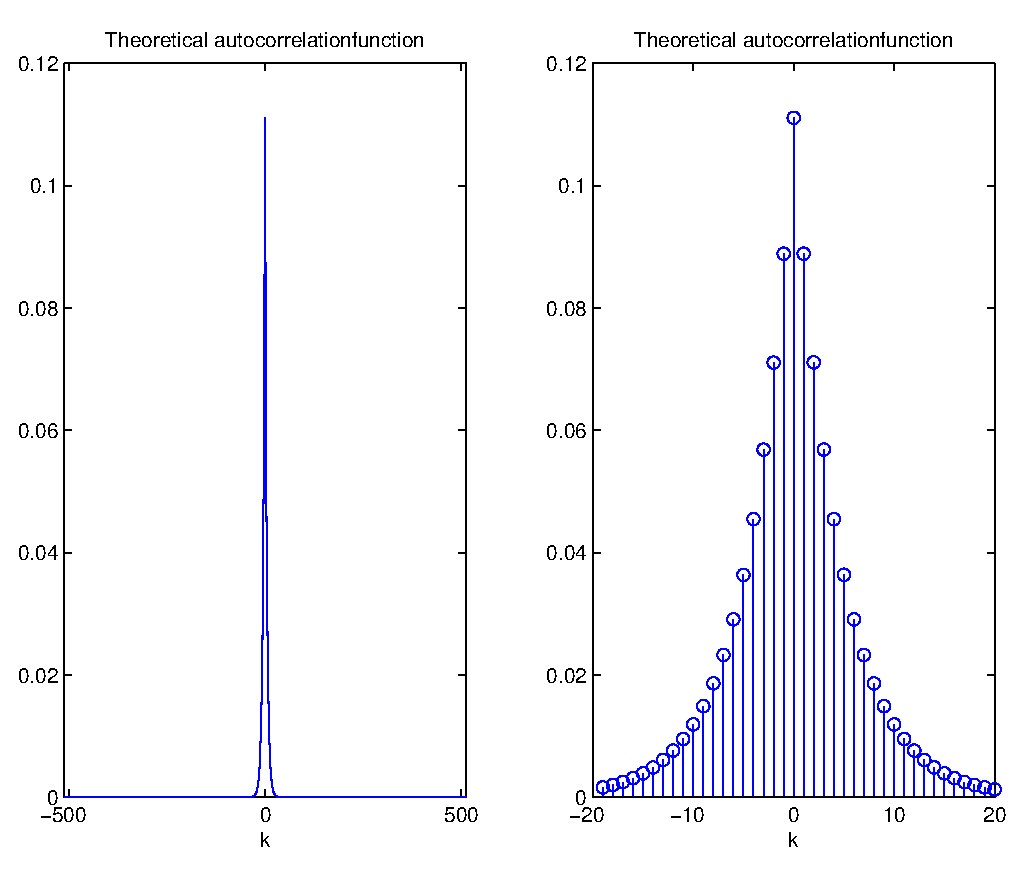
\includegraphics[width=0.6\textwidth]{TheoACF}
    \caption{Theoretical ACF of $y_{simple}$ \label{fig:TheoACFsimple}}
    \end{center}

\end{figure}

\begin{figure}[!hp]

    \begin{center}
      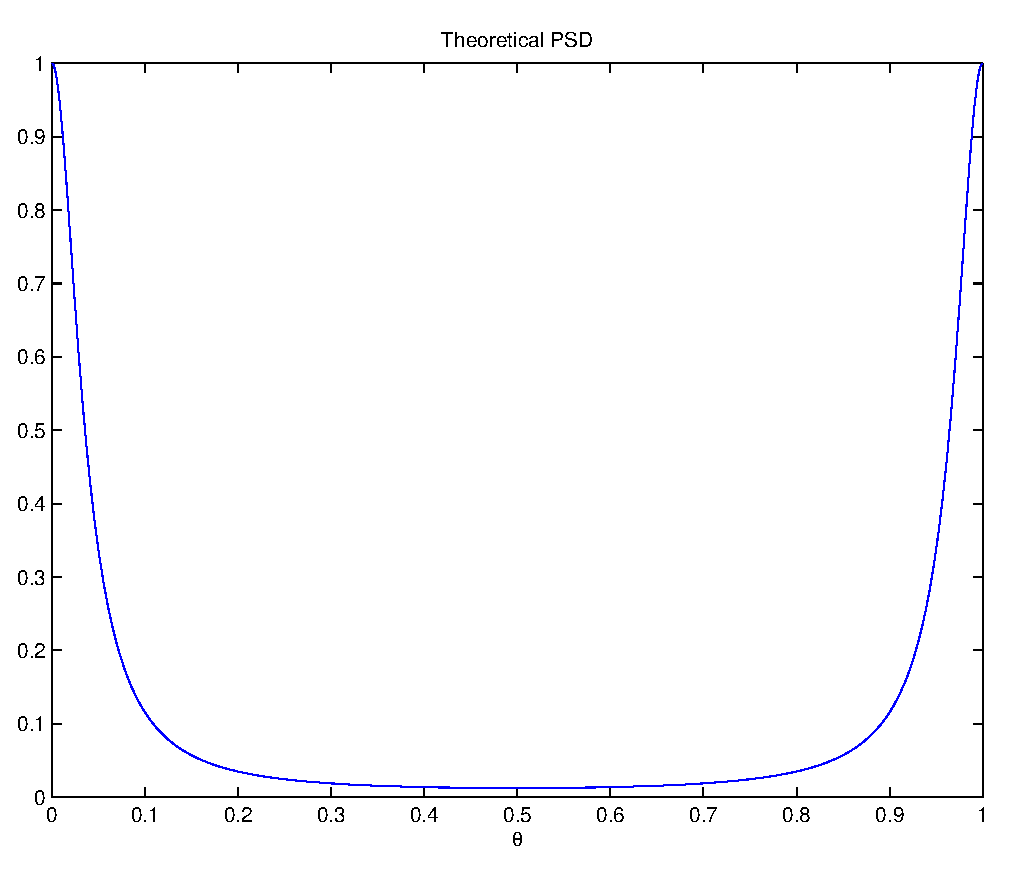
\includegraphics[width=0.6\textwidth]{TheoPSD}
    \caption{Theoretical PSD of $y_{simple}$ \label{fig:TheoPSDsimple}}
    \end{center}

\end{figure}

\begin{figure}[!hp]

    \begin{center}
      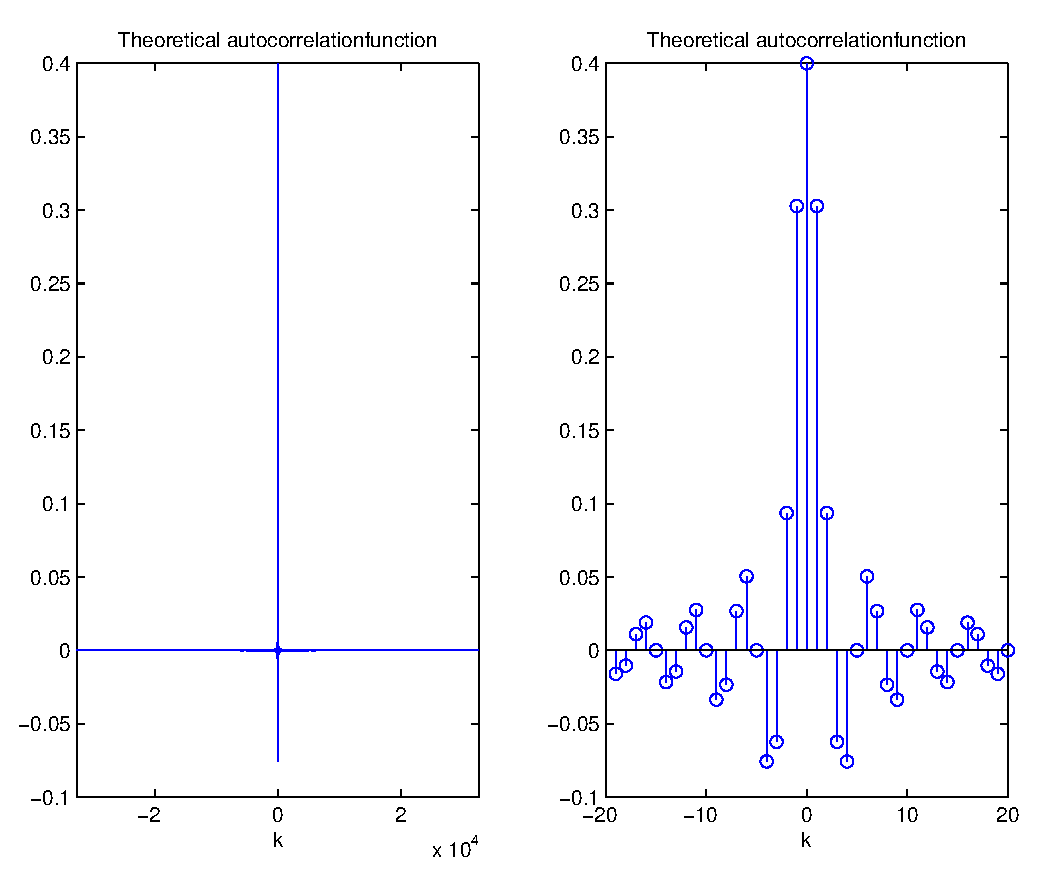
\includegraphics[width=0.6\textwidth]{BTheoACF}
    \caption{Theoretical ACF of $y_{ideal}$ \label{fig:TheoACFideal}}

    \end{center}

\end{figure}

\begin{figure}[!hp]

    \begin{center}
      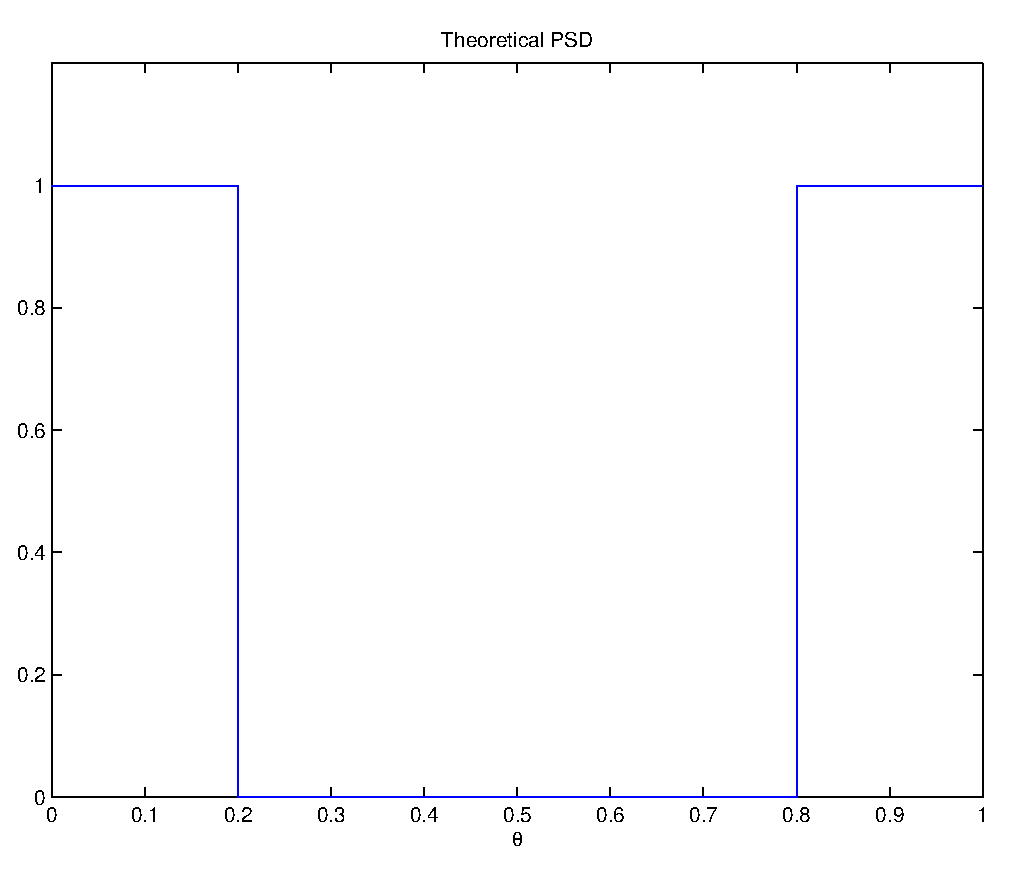
\includegraphics[width=0.6\textwidth]{BTheoPSD}
    \caption{Theoretical PSD of $y_{ideal}$ \label{fig:TheoPSDideal}}
    \end{center}

\end{figure}

\clearpage

\subsubsection{ACF estimation}

ACF estimations, of the signal filtered through the simple filter, using Blackman-
Turkey’s and Barlett’s-estimate are shown in figure~\ref{fig:ACFest}. The estimations of the signal
filtered through the near ideal filter are shown in figure~\ref{fig:BACFest}.
By examining the pictures you see the difference between the theoretical ACF and
the estimated ACF for both filters. The theoretical ACF tends to zero for higher k
while both Blackman-Turkey’s and Barlett’s-estimate are non-zero for higher k. This is
due to the fact that both Blackman-Turkey’s and Barlett’s-estimate have variances not
tending to zero for higher k. You can also see that Barlett’s estimate is slightly better
than Blackman-Turkey’s. \\


\begin{figure}[!hp]

    \begin{center}
      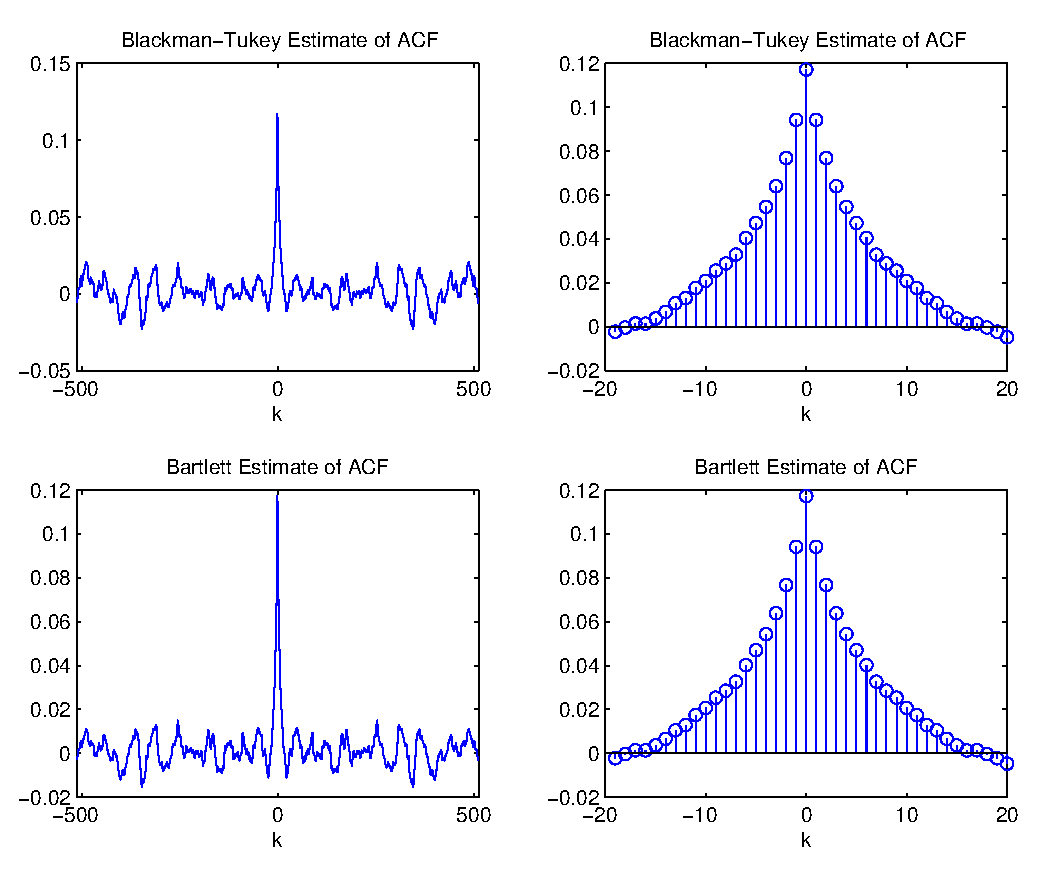
\includegraphics[width=0.6\textwidth]{EstACF}
    \caption{Estimated ACF of $y_{simple}$ \label{fig:ACFest}}
    \end{center}

\end{figure}

\begin{figure}[!hp]

    \begin{center}
      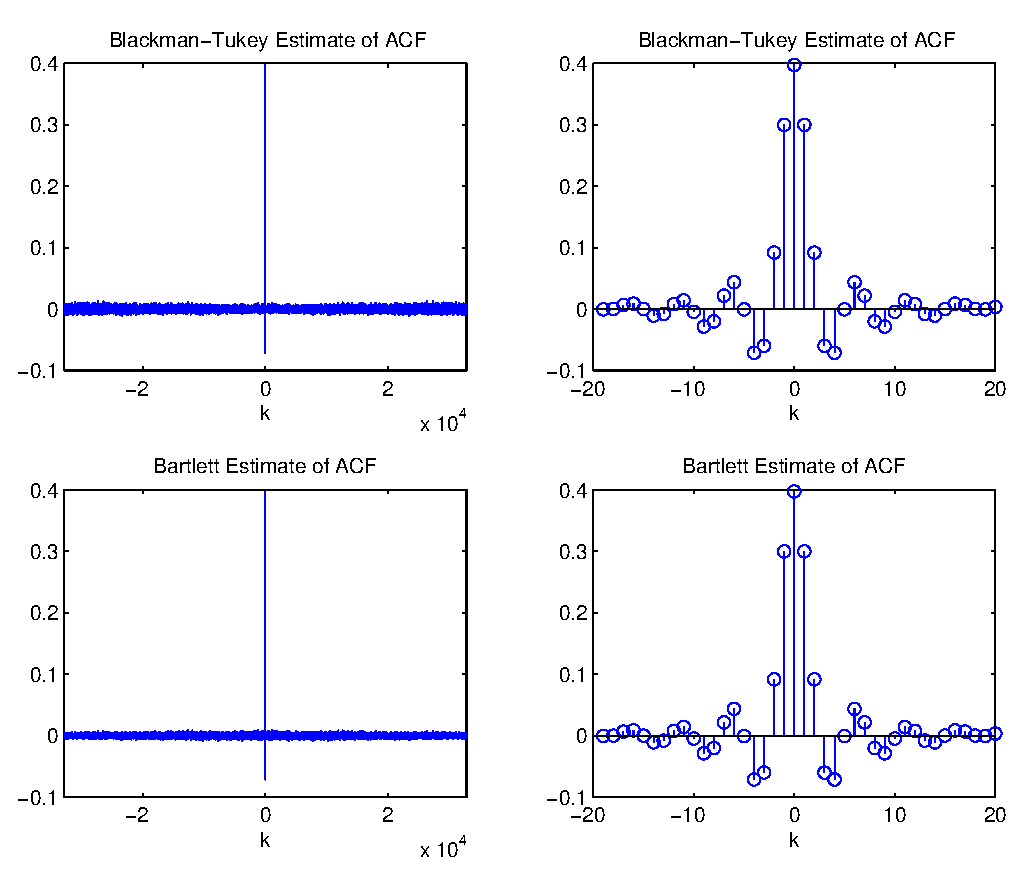
\includegraphics[width=0.6\textwidth]{BEstACF}
    \caption{Estimated ACF of $y_{ideal}$ \label{fig:BACFest}}
    \end{center}

\end{figure}

\clearpage

\subsubsection{PSD estimation}


PSD estimations of the signal filtered through the simple filter are
shown in figure~\ref{fig:PSDest} and figure~\ref{fig:PSDSmooth} while the estimations of the signal
filtered through the near ideal filter are shown in figure~\ref{fig:BPSDest} and
figure~\ref{fig:BPSDSmooth}. The raw periodogram follows the shape of the theoretical
PSD but it has a large variance. This variance was improved when using averaged periodogram,
 as can be seen in figure~\ref{fig:PSDest} and figure~\ref{fig:BPSDest}.
 However, this method sacrifices frequency resolution for a smaller variance.
 When using smoothed periodogram the variance was small and no frequency
 resolution sacrifices had to be made.


\begin{figure}[!hp]

    \begin{center}
      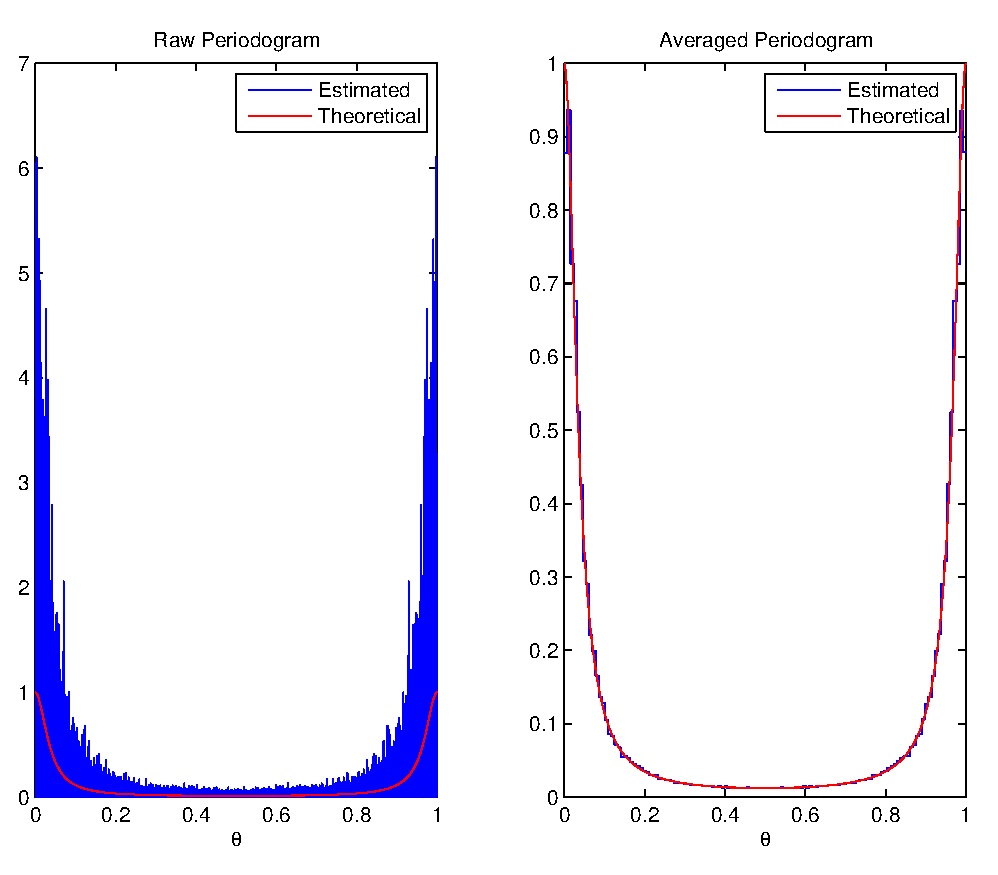
\includegraphics[width=0.6\textwidth]{Periodogram}
    \caption{Estimate PSD of $y_{simple}$ \label{fig:PSDest}}
    \end{center}

\end{figure}

\begin{figure}[!hp]

    \begin{center}
      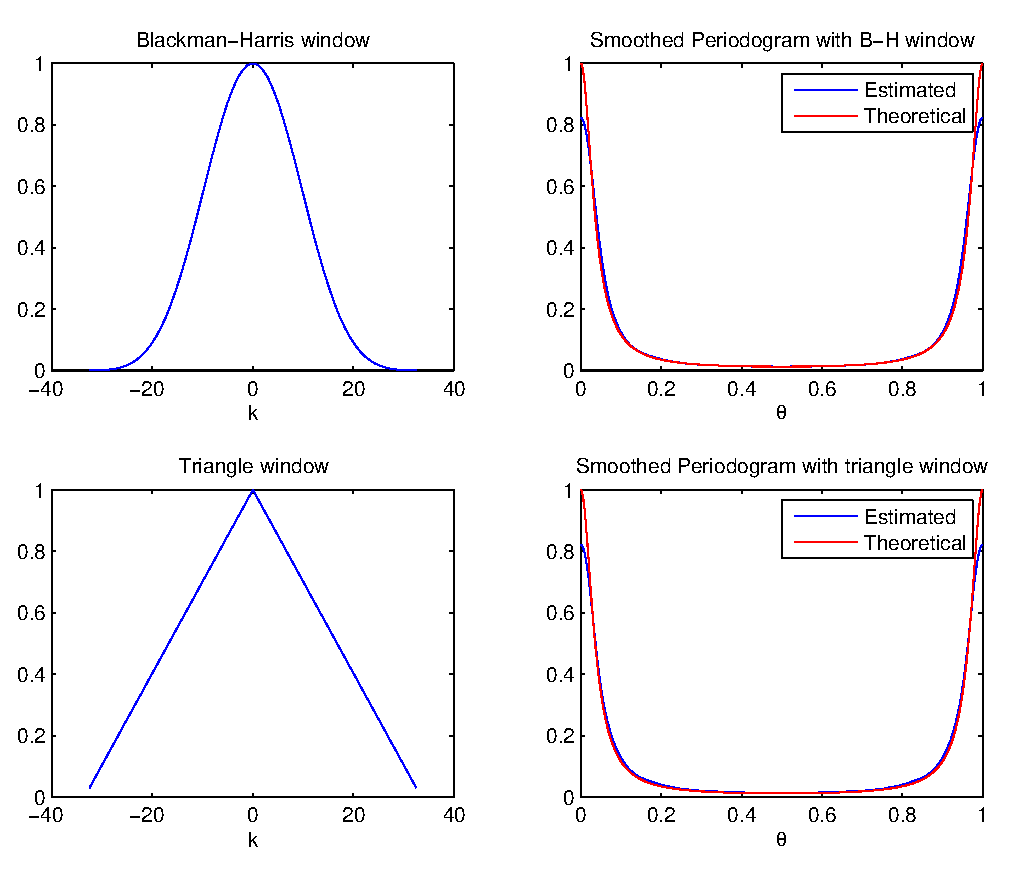
\includegraphics[width=0.6\textwidth]{Smoothed}
    \caption{Smoothed PSD of $y_{simple}$ \label{fig:PSDSmooth}}
    \end{center}

\end{figure}

\begin{figure}[!hp]

    \begin{center}
      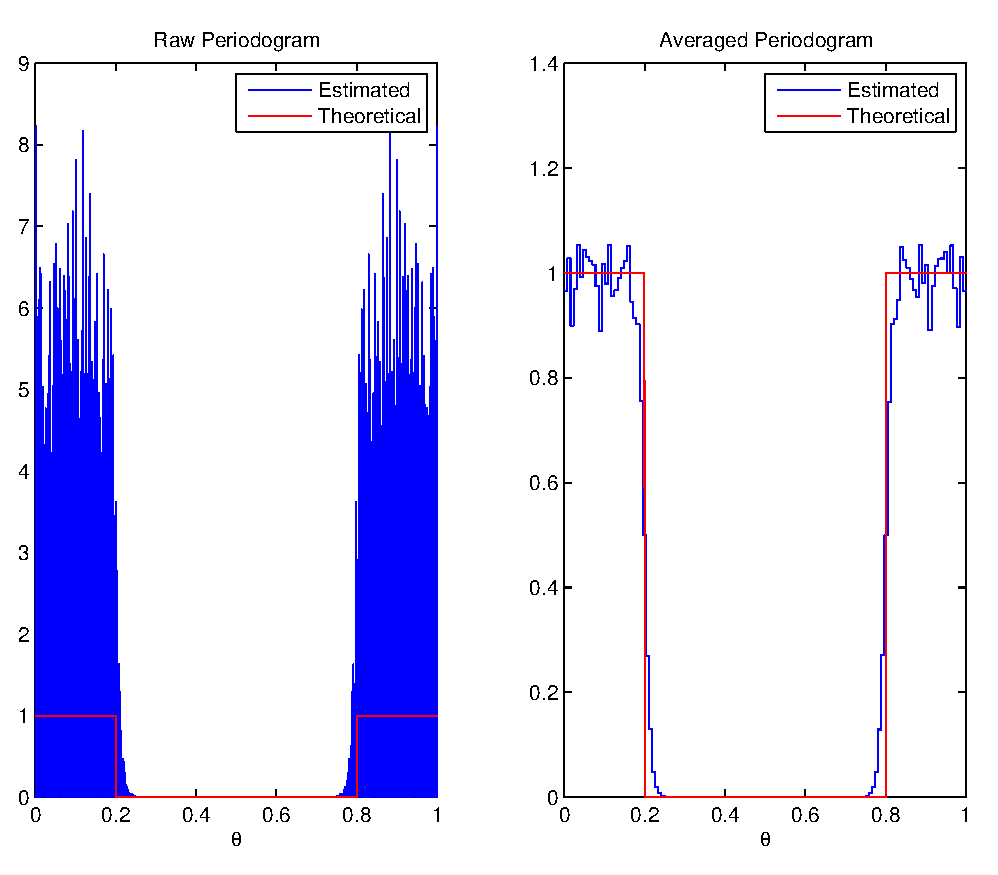
\includegraphics[width=0.6\textwidth]{BPeriodogram}
    \caption{Estimate PSD of $y_{ideal}$ \label{fig:BPSDest}}
    \end{center}

\end{figure}

\begin{figure}[!hp]

    \begin{center}
      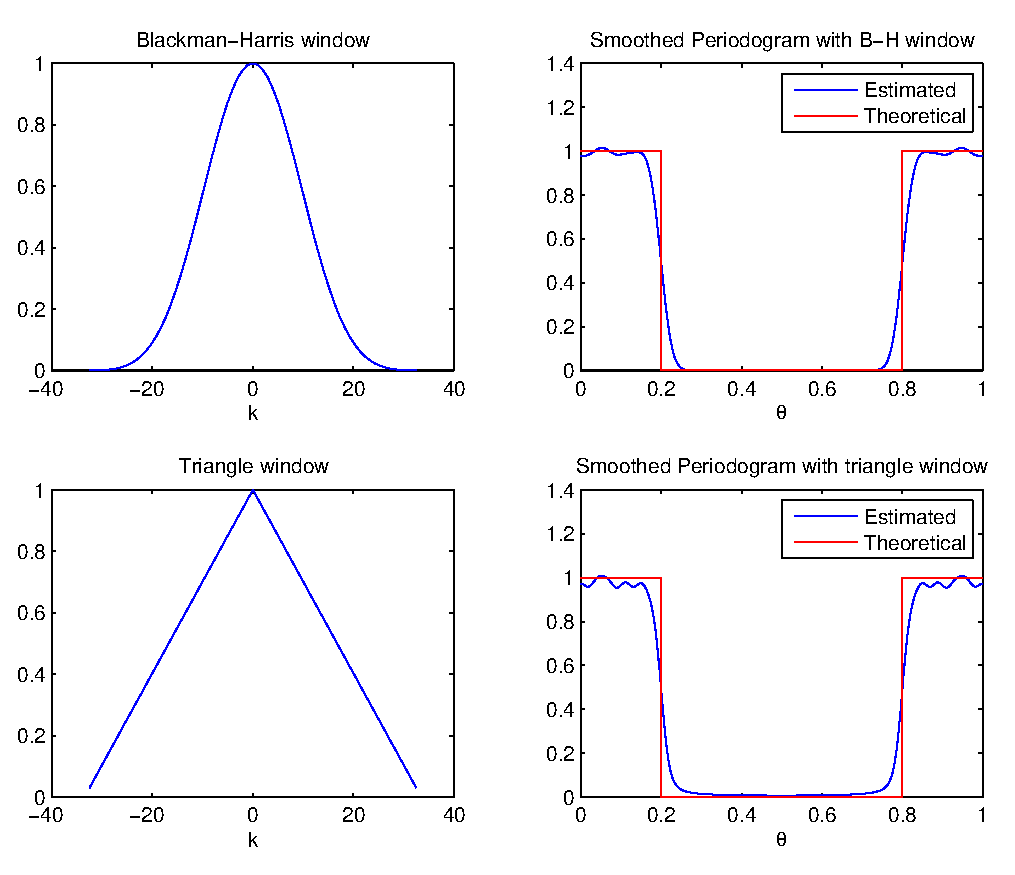
\includegraphics[width=0.6\textwidth]{BSmoothed}
    \caption{Smoothed PSD of $y_{ideal}$ \label{fig:BPSDSmooth}}
    \end{center}

\end{figure}




\clearpage


\section{Study 2 – Non-LTI-systems}
White Gaussian noise is used in this study. It was filtered through an ideal filter
described in equation~\ref{eq:idealH2} to produce the signal $x$.

\begin{equation}
  \label{eq:idealH2}
  H[\theta]_{simple} =rect(\frac{\theta} {2\theta_c})
\end{equation}

This signal, $x$, is then used as input to the three different non-LTI-systems
described in equation~\ref{eq:SQsys},~\ref{eq:HWsys} and~\ref{eq:AMsys}.
This gives the output signals $Y_{sq}$, $Y_{hw}$ and $Y_{am}$.

\begin{equation}
  \label{eq:SQsys}
  Y[n]_{sq} =X^2[n]
\end{equation}

\begin{equation}
  \label{eq:HWsys}
  Y[n]_{hw} =
\begin{cases}
   X[n],& n: X[n]>0,\\
    0,    & n: X[n] \leq 0,
\end{cases}
\end{equation}


\begin{equation}
  \label{eq:AMsys}
  Y[n]_{am} =X[n]cos(\Omega_{0}n)
\end{equation}

\subsection{Theoretical background}

Non-LTI-systems may break some properties that LTI-systems display.
Equation~\ref{eq:super} may be broken by non-LTI-systems, in other words we may
get new frequencies in our PSD when dealing with non-LTI-systems.
Gaussian input to a LTI-system has to produce a gaussian output, this does not
need to hold for non-LTI-systems.

\begin{equation}
  \label{eq:super}
  R_y[\theta] =|H[\theta]|^2R_x
\end{equation}


\subsection{Theoretical PSD}
The PSD of our filtered signal is calculated as in study 1 and the PSD formulas for our systems can be found in  \emph{Tables and formulas for signal theory, 2011, Mikael Olofsson}. The PSD's of our filtered, squared, halfwaverectified and AM-SC modulated signal
are presented in figure~\ref{fig:theoPSD2} aswell as in equation~\ref{eq:PSDfiltsig},~\ref{eq:PSDsq},~\ref{eq:PSDhw}
and~\ref{eq:PSDam}.

\begin{equation}
  \label{eq:PSDfiltsig}
   R_x[\theta] = rect[\frac{\theta} {2\theta_c}]
\end{equation}

\begin{equation}
  \label{eq:PSDsq}
  R_{sq}[\theta] = 4\theta_c\Lambda[\frac{\theta}{2\theta_c}]+4\theta_c^2\delta[\theta]
\end{equation}

\begin{equation}
  \label{eq:PSDhw}
 R_{hw}[\theta] = \frac{1}{4\pi}\Lambda[\frac{\theta}{2\theta_c}]+\frac{1}{4}rect[\frac{\theta} {2\theta_c}]
+\frac{\theta_c}{\pi}\delta[\theta]
\end{equation}

\begin{equation}
  \label{eq:PSDam}
  R_{am}[\theta] = \frac{1}{4}(rect[\frac{\theta+\Omega_{0}} {2\theta_c}]+rect[\frac{\theta-\Omega_{0}} {2\theta_c}])
\end{equation}

\begin{figure}[!hp]

    \begin{center}
      \includegraphics[width=0.6\textwidth]{TheoPSD2}
    \caption{PSD's of our systems \label{fig:theoPSD2}}
    \end{center}

\end{figure}

\subsection{Results and conclusion}

\subsubsection{Periodograms}
As we can see in figure~\ref{fig:RawPSD2} new frequencies present themselves in
the non-linear systems compared to the PSD of input, where we almost perfectly
have no frequencies between 0.1 and 0.9. All three of the non-linear systems show
frequencies between 0.1 and 0.9, even if the halfwaverectified signal doesn't do
so as clearly as the others, and thus contradicts equation~\ref{eq:super}, as can
be expected. At zero in the squared- and the halfwaverectified-
signal there is a very large spike. This is a dirac in the theoretical analysis
of the systems, but when dealing with numerical estimations this spike becomes
extremely large. The windows y-axis has been set to display the main part of the
signal instead of accomodating this large spike.


\begin{figure}[!hp]

    \begin{center}
      \includegraphics[width=0.6\textwidth]{RawPSD2}
    \caption{Estimated PSD's of our systems, with red theoretical overlay \label{fig:RawPSD2}}
    \end{center}

\end{figure}

\subsubsection{Amplitude distribution}
The input signal, in figure~\ref{fig:hist}, is the only signal that is truly gaussian in its distribution,
with the AM-SC histogram having a tendency towards gaussian but seems to have a
too high peak centered around zero. These results are expected when dealing with
non-linearities.

\begin{figure}[!hp]

    \begin{center}
      \includegraphics[width=0.6\textwidth]{Histogram}
    \caption{Histograms of our systems \label{fig:hist}}
    \end{center}

\end{figure}


\clearpage

\subsection{Study 3 – Special Operations}
The input signal from study 2, $x$m is used as input signal in this study too. It consists of
filtered white Gaussian noise and is used as inputs to systems described in equation ~\ref{eq:alt}
and ~\ref{eq:dec}. This gives the output signals $Y_{alt}$ and $Y_{dec}$.

\begin{equation}
  \label{eq:alt}
  Y[n]_{alt} =X[n](-1)^n
\end{equation}

\begin{equation}
  \label{eq:dec}
  Y[n]_{dec} =
\begin{cases}
   X[n],& for~even~n\\
    0,    & for~odd~n
\end{cases}
\end{equation}

\subsection{Realizing the systems}
In order du calculate the PSD as simply as possible we used cosine to rewrite our systems as described
in ~\ref{eq:alt2} and ~\ref{eq:dec2}.

\begin{equation}
  \label{eq:alt2}
  Y[n]_{alt} =X[n]cos(\pi n)
\end{equation}

\begin{equation}
  \label{eq:dec2}
  Y[n]_{dec} =\frac{1}{2}X[n](1+cos(\pi n))
\end{equation}

The system in~\ref{eq:alt2} describes the same alternating system as equation~\ref{eq:alt} and
the system in~\ref{eq:dec2} describes the same decimating system as equation~\ref{eq:dec}.
By ocular inspection we see that equation~\ref{eq:alt} describes a amplitude modulation with 
suppressed carrier, amplitude constant $1$ and carrier frequency $0.5$. In turn equation~\ref{eq:dec}
describes a demodulation with amplitude constant $0.5$ and carrier frequency $0.25$.

\subsection{Theoretical PSD}

Since the systems can be described as a modulation and demodulation the corresponding equations
for the PSD's can be found in \emph{Signal Theory, 2011, Mikael Olofsson}. This gives us the
equations~\ref{eq:PSDalt} and~\ref{eq:PSDdec}. Where $R_X$ can be found in equation~\ref{eq:RX}.
In equation~\ref{eq:PSDalt}, $\theta_c$ will be 0.5, this means that the two
resulting rectangular functions will overlap. A similar thing happens in
equation~\ref{eq:PSDdec} as well.

\subsection{Result and conclusion}

\begin{equation}
  \label{eq:RX}
  R_{X} = rect(\frac{\theta}{2\theta_0} )
\end{equation}

\begin{equation}
  \label{eq:PSDalt}
  R_{alt} = \frac{1}{4}(R_X(\theta+\theta_c) + R_X(\theta-\theta_c)) = \Bigg/ \theta_c = \frac{1}{2} \Bigg/ = \frac{1}{2}(R_X(\theta-\frac{1}{2}))
\end{equation}

\begin{align}
  \label{eq:PSDdec}
  R_{dec} & = \frac{1}{2^2}R_X(\theta) + \frac{1}{2^2}\frac{1}{4}(R_X(\theta+2\theta_c)
  + R_X(\theta-2\theta_c)) \\
   & = \Bigg/ \theta_c  = \frac{1}{4} \Bigg/ = \nonumber
   \frac{1}{4}R_X(\theta) + \frac{1}{8}R_X(\theta-\frac{1}{2})
\end{align}


\subsection{Results and conclusion}

As we can see in figure~\ref{fig:PSD3} the estimated PSD's are approximated
quite nicely, this effect is even more clearly visible when the PSD's are smoothed
with a Blackman-Harris window of size 65 as we can see in figure~\ref{fig:PSD3smooth}
It's interesting to note that a alternating sampling of a signal corresponds to
a amplitude modulation with suppressed carrier and that a decimation can be seen
as the demodulation with scaled amplitude.

\begin{figure}[!hp]

    \begin{center}
      \includegraphics[width=0.6\textwidth]{PSD3}
    \caption{PSD of input and the two outputs \label{fig:PSD3}}
    \end{center}

\end{figure}

\begin{figure}[!hp]

    \begin{center}
      \includegraphics[width=0.6\textwidth]{PSD3smooth}
    \caption{Smoothed PSD of input and the two outputs\label{fig:PSD3smooth}}
    \end{center}

\end{figure}

\end{document}
